\documentclass[Modultest/Modultest_main.tex]{subfiles}
\begin{document}
\section{Cup Sensor} \label{sec:CupSensor}
Der udføres en modultest som tester både, hardware blokken Cup Sensor og software klassen CupSensor\_IF. Dette er ikke nødvendigvis den mest rigtige måde at udføre modultest på. Den vigtige grænseflade til sensoren er i softwaren mellem controllerklassen GameController og CupSensor\_IF på PlayerSideApp. Hardwaren og softwaren blev også udviklet parralelt med hinanden, og der er derfor ikke specificeret en detaljeret hardware grænseflade, da dette ikke er så vigtigt. Derfor anses det som værende acceptabelt at udføre modultest af hardware og software samtidig.

\subsection{Krav der testes}
Cup sensoren formål er at detektere at en cup er placeret eller ej, samt at detektere at en bold rammer i koppen. Til at teste sensoren udvælges de relvevante dele fra kravspecifikation og arkitekturen. Der er fra kravspecifikationen nedenstående krav til sensoren
\begin{enumerate}
    \item \textbf{K\ref{kravspec:req:beer-amount}} Systemet skal fungere med $110\si{ml} \pm 20\si{ml}$ Ceres Top øl i hver Cup.
    
    \item  \textbf{K\ref{kravspec:req:ball-color}} Systemet skal fungere med en almindelig hvid bordtennis bold
    
    \item  \textbf{K\ref{kravspec:req:ball-drop-height}} Systemet skal detektere en bold der falder fra en højde på 30cm over bordet.
    
    \item \textbf{K\ref{kravspec:req:max-cup-offset}} Systemet skal detektere placering af en Cup når centrum af Cup og centrum af CupHolder er under 10mm
    
    \item  \textbf{K\ref{kravspec:req:placed-succes-rate}} Det skal detekteres 99 ud af 100 gange at der placeres en \textbf{Cup} i en kopholder. 
    
    \item \textbf{K\ref{kravspec:req:removed-succes-rate}} Det skal detekteres 99 ud af 100 gange at der løftes en \textbf{Cup} fra en kopholder. 
    
    \item \textbf{K\ref{kravspec:req:dropped-succes-rate}} Det skal detekteres 95 ud af 100 gange at en \textbf{Ball} rammer i  en \textbf{Cup} som står i en kopholder.
    
    \item \textbf{K\ref{kravspec:req:hour-false-placed}} I en periode på 1 time uden ydre påvirkninger af systemet må der højest være 1 falsk detektering af placering af en \textbf{Cup} på tom kopholder.
    
    \item \textbf{K\ref{kravspec:req:hour-false-removed}} I en periode på 1 time uden ydre påvirkninger af systemet må der højest være 1 falsk detektering af løfting af en \textbf{Cup} fra kopholder hvor der står en kop.
    
    \item \textbf{K\ref{kravspec:req:ball-hit-sensor-false-placed}} Når en \textbf{Ball} rammer en kopholder og hopper væk igen 100 gange (uden nogen \textbf{Cup}) må der højest ske 1 falsk detektering af at der placeres en \textbf{Cup} i den givne kopholder.
\end{enumerate}

For at teste disse krav laves der forskellige måleserier. Alle måleserier udføres med Ceres Top øl (\textbf{K\ref{kravspec:req:beer-amount}}). Alle måleserier gentages med 90ml, 110ml og 130ml øl (\textbf{K\ref{kravspec:req:beer-amount}}), for at teste den øvre og nedre grænse af mængden af øl, samt den specificerede mængde øl (110ml). Hvis sensoren består testen med disse mængder øl, antages det at den også vil virke i hele intervallet mellem 90ml og 130ml. Alle måleserier benytter en hvid bold (\textbf{K\ref{kravspec:req:ball-color}}). Ved alle måleserier der involverer detektering af at en bold rammer i, tabes boldens centrum fra 30cm over bordet (\textbf{K\ref{kravspec:req:ball-drop-height}}). Der udføres forskellige måleserier til at måle pålideligheden af sensoren (\textbf{K\ref{kravspec:req:placed-succes-rate}}, \textbf{K\ref{kravspec:req:removed-succes-rate}} og \textbf{K\ref{kravspec:req:dropped-succes-rate}}). Der udføres måleserier hvor der ventes en time og der noteres hvor mange falske detekteringer der forekommer (\textbf{K\ref{kravspec:req:hour-false-removed}} og \textbf{K\ref{kravspec:req:hour-false-removed}}). Der udføres måleserier hvor en bold rammer sensoren og hopper væk igen 100 gange (\textbf{K\ref{kravspec:req:ball-hit-sensor-false-placed}}).

Der er fra arkitekturen nedenstående krav til sensoren.
\begin{enumerate}
    \item Skal fungere med en forsyningsspænding på $5.0\si{V} \pm 0.2\si{V}$ \label{itm:supply_voltage}
    \item Skal kalde metoden updateCupStatus når en kop fjernes og placeres \label{itm:update_cup_function}
    \item Skal kalde metoden updateHitStatus når en kop rammes af en bold. \label{itm:update_hit_function}
\end{enumerate}

For at teste disse krav udføres forskellige måleserier. Alle de førnævnte måleserier gentages ved en forsyningsspændinger på 4.8V, 5.0V og 5.2V (punkt \ref{itm:supply_voltage}), for at teste den øvre og nedre grænse af forsyningsspændingen, nominielle forsyningsspænding (5.0V). Hvis sensoren består testen med disse forsyningsspændinger, antages det at den også vil virke i hele intervallet mellem 4.8V og 5.2V. Til alle måleserier benyttes et testprogram som kræver at de to funktioner updateCupStatus og updateHitStatus bliver kaldt. Hvis disse ikke bliver kaldt, er der ingen måleserier der vil virke (punkt \ref{itm:update_cup_function} og \ref{itm:update_hit_function}).

\subsection{Testopstilling}
Der benyttes to forskellige testopstillinger.
Til de fleste test benyttes test opstillingen som ses på figur \ref{fig:testOneSensor}. Der benyttes (den første udgave af) printpladen for Cup Holder men kun Cup Sensor delen benyttes. Der er desuden på et fumlebræt implementeret RC ledet (lavpasfilteret) som er beskrevet i Hardware design dokumentet. 

\begin{figure}[H]
    \centering
    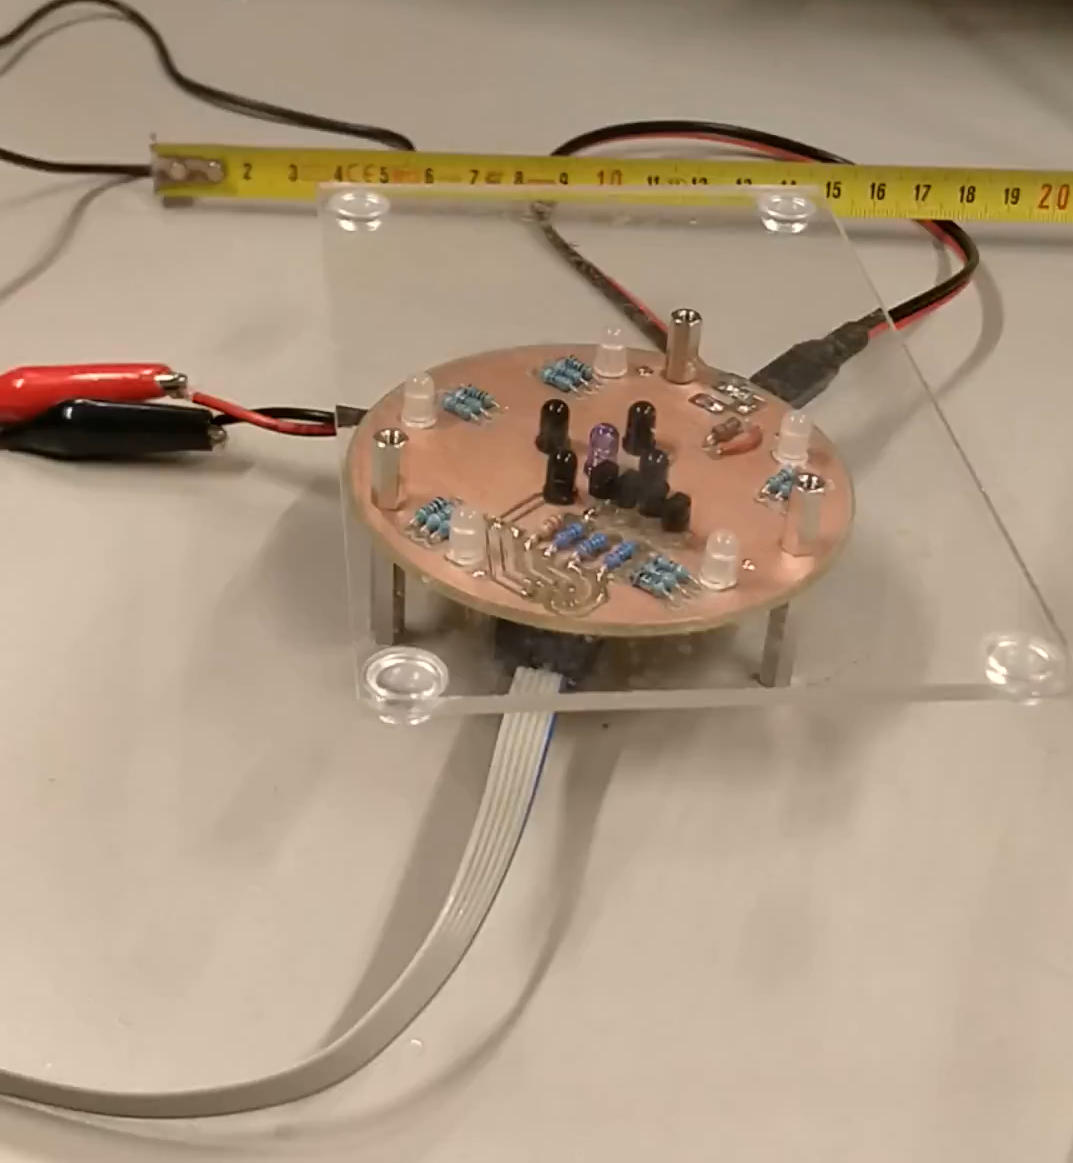
\includegraphics[width=0.8\textwidth]{Modultest/CupSensor/testOpstilling/testOneSensor.png}
    \caption{Opstilling hvor der benyttes en sensor. D}
    \label{fig:testOneSensor}
\end{figure}

Til måleserierne hvor der tabes en bold i koppen, HW og SW mæsigt den samme opstilling som tidligere beskrevet, men der benyttes et målebånd som ses på figur \ref{fig:testBallDrop}. Her indstilles målebåndet til at enden af målebåndet er 30 cm over plastikpladen. I udførelsen af måleserierne tabes bolden når dens centrum er i enden af målebåndet, som det ses i toppen af \ref{fig:testBallDrop}.

\begin{figure}[H]
    \centering
    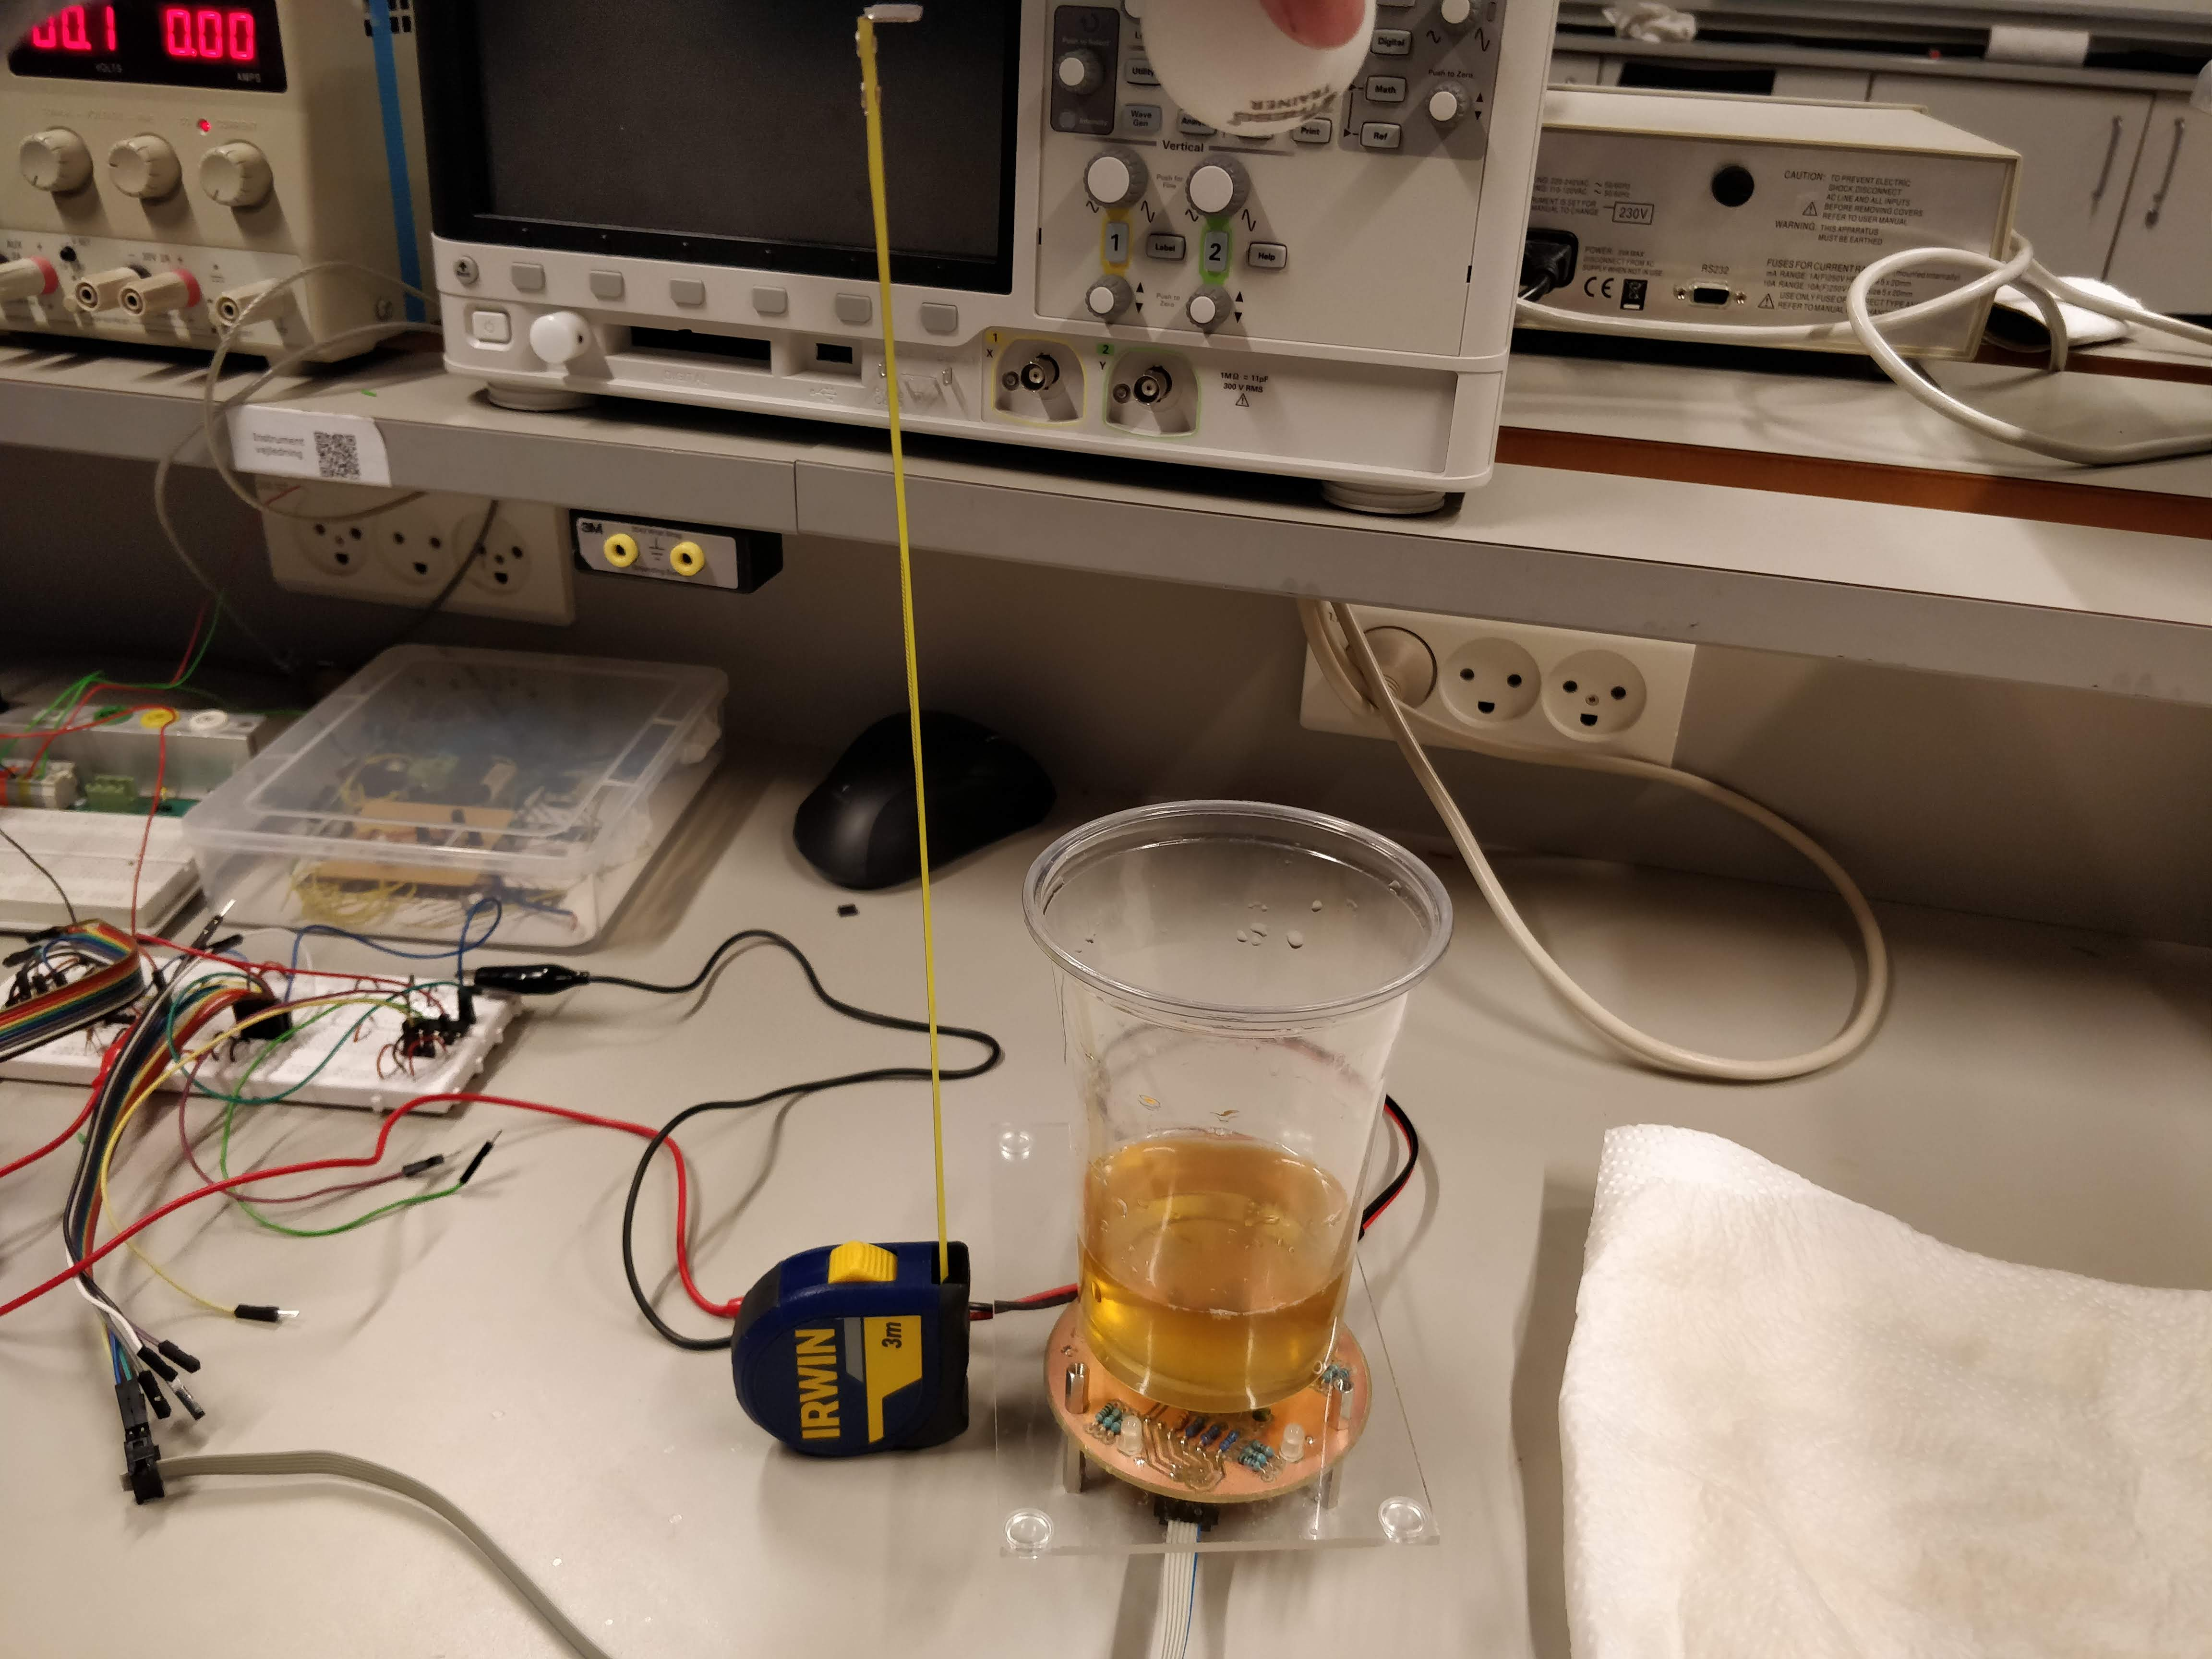
\includegraphics[width=0.8\textwidth]{Modultest/CupSensor/testOpstilling/testBallDrop.jpg}
    \caption{Opstilling til måling hvor der tabes en bold}
    \label{fig:testBallDrop}
\end{figure}

Til testene hvor der skal ventes i en time, benyttes der opstillingen som ses på figur \ref{fig:testMoreSensors}. Dette er valgt så der kan testes både falske detekteringer af placering af kom og falske detekteringer af fjernelse af kop. Derudover tænkes det også at sensorerne muligvis kan påvirke hinanden, dette testes derfor også som en del af denne testopstilling. Der benyttes desuden Cup Holder Controller Veroboardet som en del af denne opstilling. For at de andre dele ikke påvirker denne modultest, fjernes IC'erne der styre Cup Light. Der benyttes desuden en nyere version af printpladen men der er ikke nogen markant forskel.
\begin{figure}[H]
    \centering
    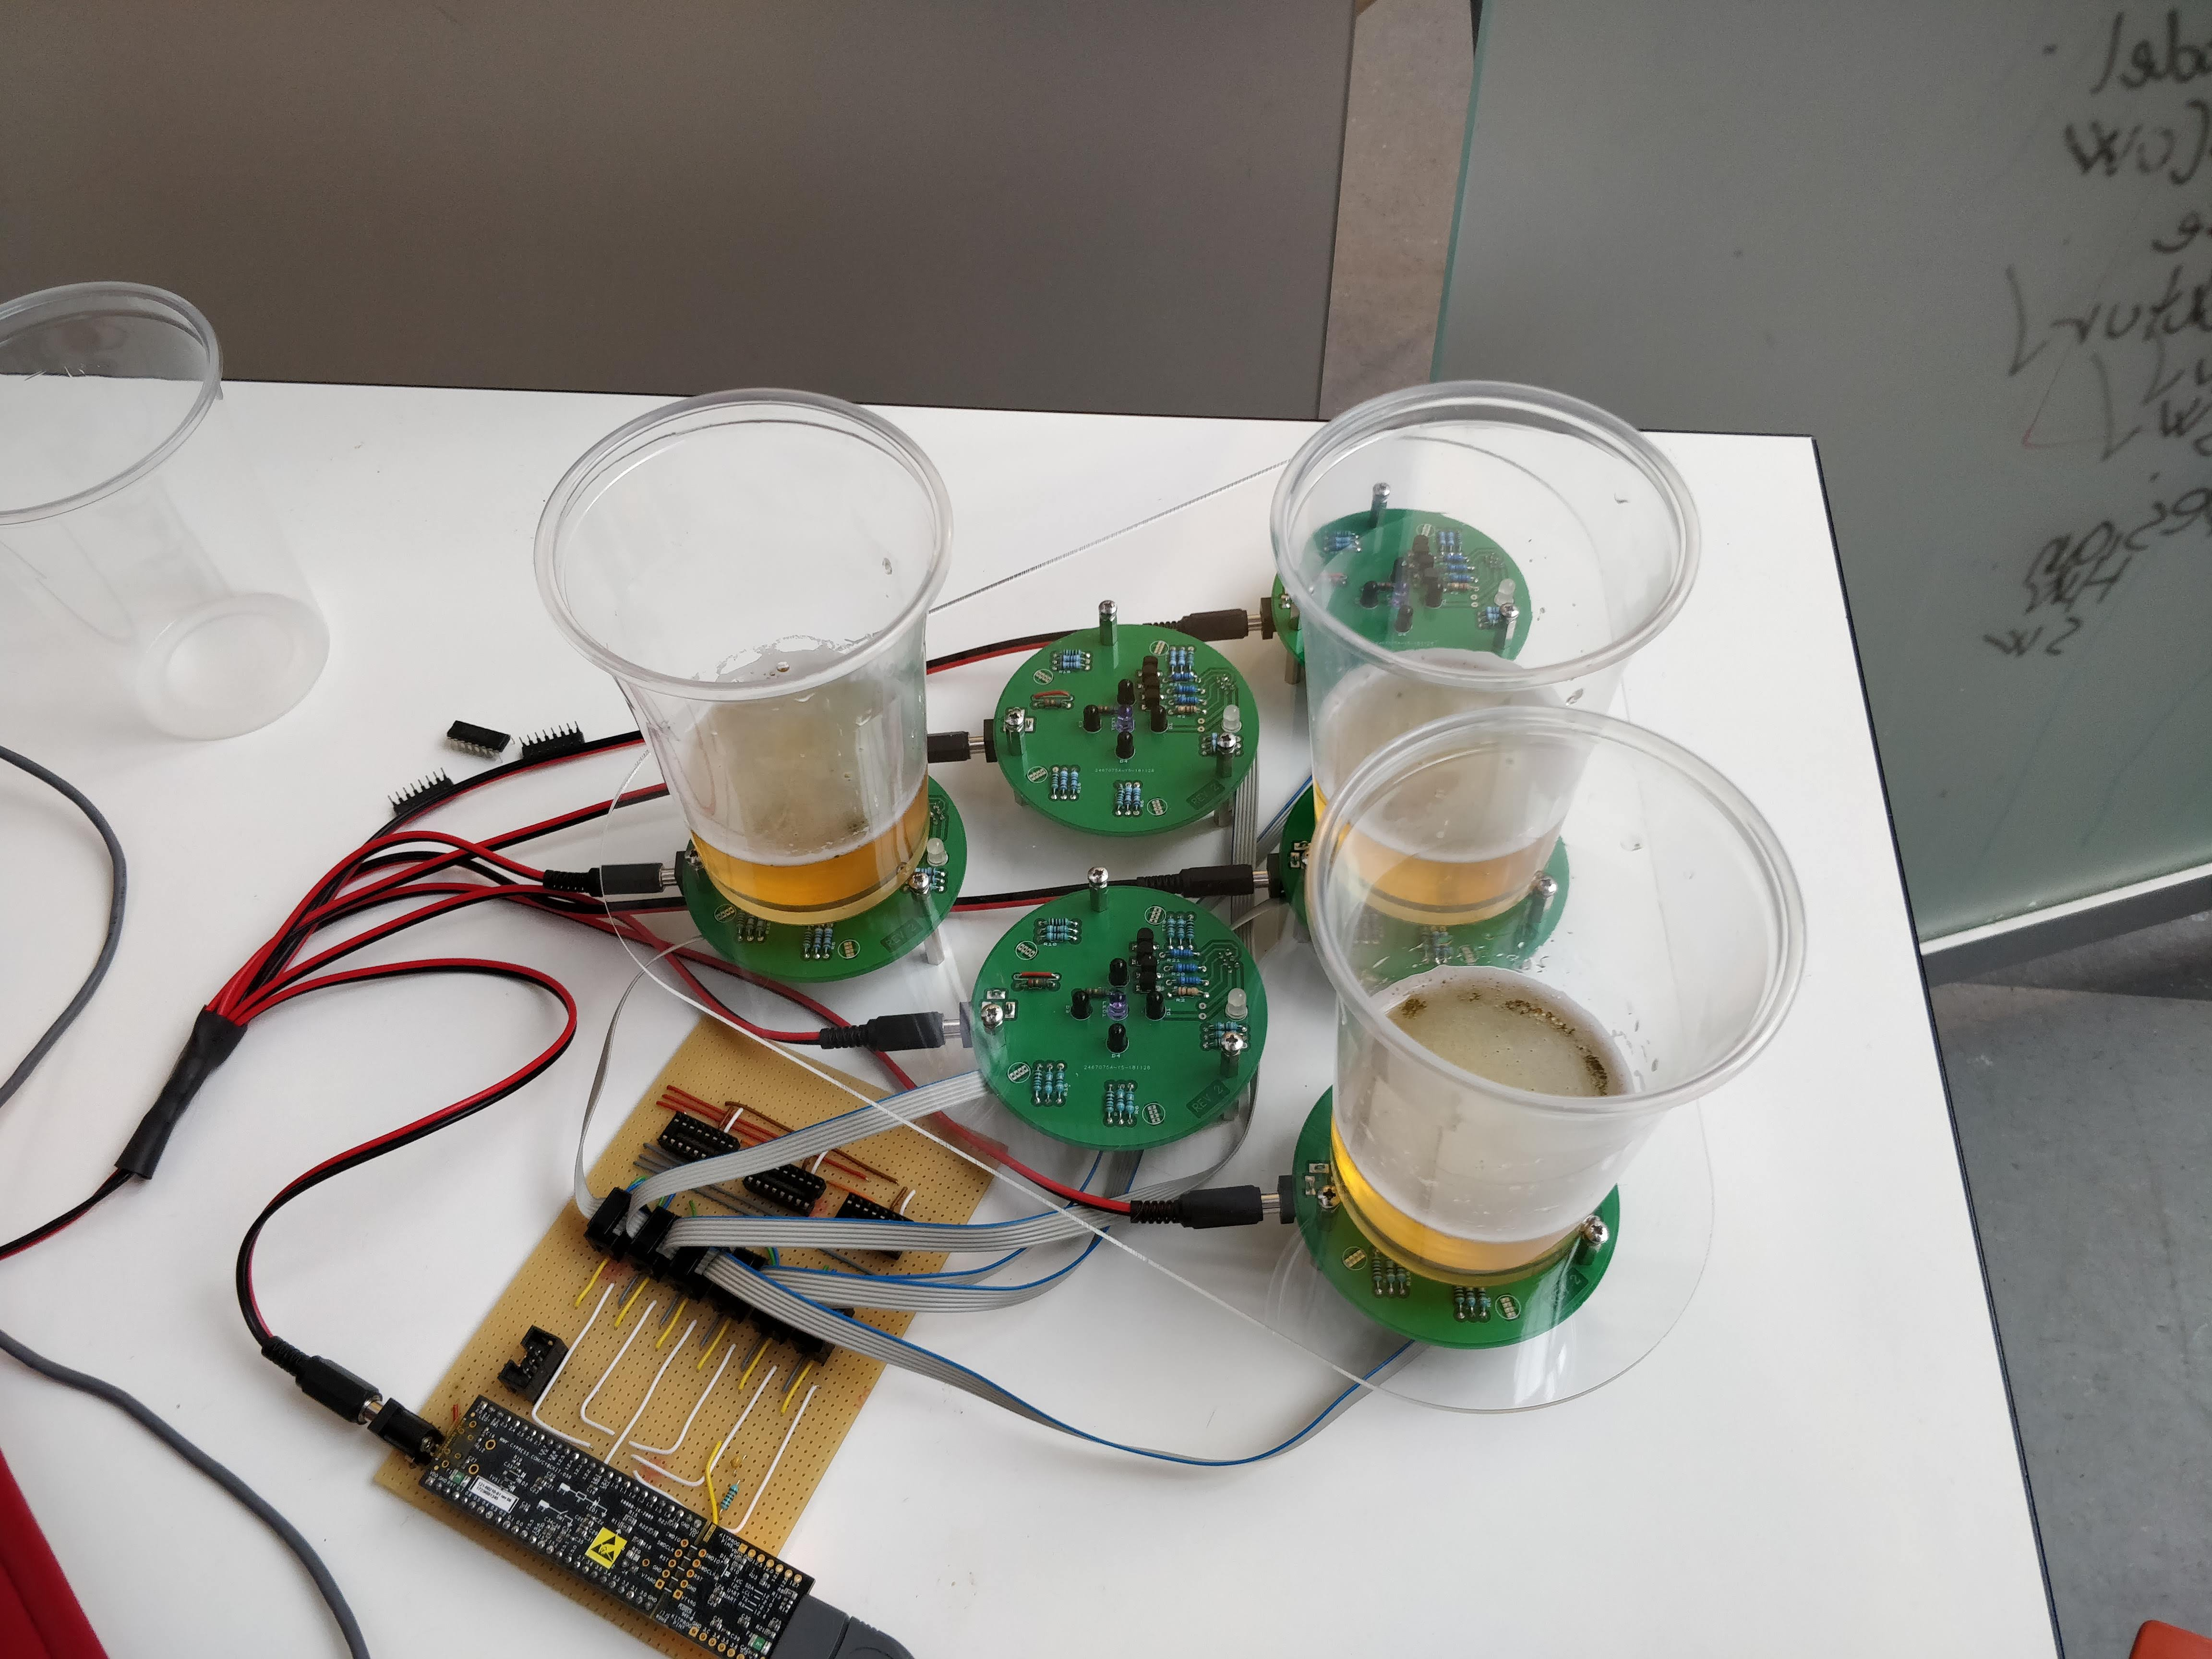
\includegraphics[width=1\textwidth]{Modultest/CupSensor/testOpstilling/testMoreSensors.jpg}
    \caption{Opstilling hvor der benyttes en 6 sensorer.}
    \label{fig:testMoreSensors}
\end{figure}

Til begge opstillinger bruges programmet som ses på listing. Programmet tæller hvor mange gange der placeres og fjernes en kop. Den tæller også hvor mange gange en bold rammer i. Hver gang der sker en ændring udskrives antallet af alle disse tælleværdier vha. en UART komponent som er er del af testprogrammet. \ref{lis:CupSensorTestProgram}
\lstinputlisting[language=C, firstline=5, lastline=42,style=customc,caption={Udsnit af testprogram. },label=lis:CupSensorTestProgram]{Modultest/CupSensor/testApp/main.c}

\subsection{Målinger}
For at teste pålideligheden for detektering af placering af kop og fjernelse af kop (\textbf{K\ref{kravspec:req:placed-succes-rate}} og \textbf{K\ref{kravspec:req:removed-succes-rate}}), laves der en måleserie hvor der placeres en kop og derefter fjernes den igen 100 gange. Testprogrammet tæller hvor mange gange en kop placeres, fjernes og rammes af en bold. Hvis der sker en fejl som at der fx. ikke detekteres en at en kop bliver fjernet, fremprovokeres en detektion af fjernelse af kop og ændringer i testprogrammet tælleværdier noteres for resultaterne kompenseres for dette. Resultaterne ses nedenfor. Måleserien gentages som tidligere beskrevet med 90ml, 110ml og 130ml, disse måleserie udføres ved 4.8V, 5.0V og 5.2V. Så i alt 9 måleserier. Resultatet kan ses på \ref{tab:100_placed_removed_cups}
\begin{table}[H]
    \centering
    \begin{tabular}{|L{0.15\textwidth}|L{0.15\textwidth}|L{0.2\textwidth}|L{0.2\textwidth}|L{0.2\textwidth}|}
         \hline
         \textbf{Øl volumen} & \textbf{Spænding} & \textbf{Antal placering} & \textbf{Antal fjernelser} & \textbf{Antal bolde} \\ \hline
         90ml & 4.8V & 100 & 100 & 0 \\ \hline 
         90ml & 5.0V & 100 & 100 & 0 \\ \hline 
         90ml & 5.2V & 100 & 100 & 0\\ \hline
         110ml & 4.8V & 100 & 100 & 0 \\ \hline 
         110ml & 5.0V & 100 & 100 & 0 \\ \hline 
         110ml & 5.2V & 100 & 100 & 0 \\ \hline
         130ml & 4.8V & 100 & 100 & 0 \\ \hline 
         130ml & 5.0V & 100 & 100 & 0\\ \hline 
         130ml & 5.2V & 100 & 100 & 0 \\ \hline
    \end{tabular}
    \caption{Måling af placering og fjernelse af 100 kopper}
     \label{tab:100_placed_removed_cups}
\end{table}


For at teste pålideligheden for detektering af at en bold rammer i (\textbf{K\ref{kravspec:req:dropped-succes-rate}}), udføres en måleserie hvor der tabes tabes en bold 100 gange med en højde på 30cm over bordoverfladen. Det detekteres hvor mange gange dette detekteres vha. testprogrammet. Der udføres ligesom før en måleserie med 90ml, 110ml og 130ml. Disse tre måleserie udføres for en forsyningsspænding på 4.8V, 5.0V og 5.2V. Igen i alt 9 måleserier. 
Disse måleserier er ikke helt ideele da mængden af øl formindskes mellem hver gang bolden tabes. Der kan være noget som sprøjter ud af koppen, og hovedsagligt vil der være øl tilbage på bolden når den tages ud. Man burde derfor at genopfylde koppen til den nødvendige mængde øl, mellem hver gang bolden tabes. Da dette vil tage lang tid, genopfyldes koppen kun mellem hver måleserie. Resultatet kan ses på \ref{tab:100_hit_cup}
\begin{table}[H]
    \centering
    \begin{tabular}{|L{0.15\textwidth}|L{0.15\textwidth}|L{0.2\textwidth}|}
         \hline
         \textbf{Øl volumen} & \textbf{Spænding} & \textbf{Antal detekteringer} \\ \hline
         90ml & 4.8V & 96 \\ \hline 
         90ml & 5.0V & 100 \\ \hline 
         90ml & 5.2V & 98 \\ \hline
         110ml & 4.8V & 97\\ \hline 
         110ml & 5.0V & 100 \\ \hline 
         110ml & 5.2V & 100\\ \hline
         130ml & 4.8V & 99\\ \hline 
         130ml & 5.0V & 93\\ \hline 
         130ml & 5.2V & 85\\ \hline
    \end{tabular}
    \caption{Måling af tab af bold 100 gange}
     \label{tab:100_hit_cup}
\end{table}

For at teste hvor mange falske detekteringer der er når en bold rammer sensoren uden nogen kop (\textbf{K\ref{kravspec:req:ball-hit-sensor-false-placed}}), udføres en måleserie hvor en bold kastes på sensoren hvorefter den hopper væk. Dette udføres 100 gange. Der tælles vha. testprogrammet hvor mange detekteringer af placering af kop der kommer.  Denne måleserie gentages ved forsyningsspændingerne 4.8V, 5.0V og 5.2V. Resultatet kan ses på \ref{tab:100_hit_sensor}.

\begin{table}[H]
    \centering
    \begin{tabular}{|L{0.15\textwidth}|L{0.2\textwidth}|}
         \hline
         \textbf{Spænding} & \textbf{Antal detekteringer af placering af kop} \\ \hline
         4.8V &  0\\ \hline 
         5.0V &  0\\ \hline 
         5.2V &  0\\ \hline
    \end{tabular}
    \caption{Måling af bold som rammer sensor 100 gange}
     \label{tab:100_hit_sensor}
\end{table}

For at teste hvor mange falske detekteringer af placering og fjernelse af en kop der sker på en time (\textbf{K\ref{kravspec:req:placed-succes-rate}} og \textbf{K\ref{kravspec:req:removed-succes-rate}}), udføres en måleserie hvor der i en time ikke står en kop på 3 sensorer og der står en kop på de 3 andre. Det tælles vha. testprogrammet hvor mange falske detekteringer af placering af kop der kommer. Dette udføres kun ved en forsyningsspænding på 5V, pga. tidsmangel. Resultatet kan ses på \ref{tab:1_hour}.

\begin{table}[H]
    \centering
    \begin{tabular}{|L{0.15\textwidth}|L{0.2\textwidth}|L{0.2\textwidth}|L{0.2\textwidth}|}
         \hline
         \textbf{Spænding} & \textbf{Antal detekteringer af placering af kop} & \textbf{Antal fjernelser} & \textbf{Antal bolde der rammer i} \\ \hline
         5.0V & 0 & 0 & 0\\ \hline
    \end{tabular}
    \caption{Måling af 3 sensorer uden nogen kop og 3 sensorer med en kop i en time}
     \label{tab:1_hour}
\end{table}

\subsection{Konklusion}
Det kan konkluderes at \textbf{K\ref{kravspec:req:placed-succes-rate}} og \textbf{K\ref{kravspec:req:removed-succes-rate}} er opfyldt, da det med alle mængder øl og alle forsyningsspændinger detekteres at der placeres og fjernes en kop 100 ud af 100 gange. Kravet er 99 ud af 100 gange. 
Det kan konkluderes at \textbf{K\ref{kravspec:req:dropped-succes-rate}} ikke er opfyldt, da der, med 130ml øl og en forsyningsspænding på 5.0V og 5.2V, kun detekteres at en bold rammer i 93 og 85 ud af 100 gange. Kravet er 95 ud af 100 gange.

Det kan konkluderes at \textbf{K\ref{kravspec:req:hour-false-placed}} og \textbf{K\ref{kravspec:req:hour-false-removed}} er opfyldt, da der på en time ikke sker nogen falske detekteringer af nogen type.

Det kan konkluderes at \textbf{K\ref{kravspec:req:ball-hit-sensor-false-placed}} er opfyldt da der ikke sker nogen falske detekteringer når bolden rammer sensoren.

Da  \textbf{K\ref{kravspec:req:dropped-succes-rate}} ikke er opfyldt, er \textbf{K\ref{kravspec:req:beer-amount}}, \textbf{K\ref{kravspec:req:ball-color}} og  \textbf{K\ref{kravspec:req:ball-drop-height}} derfor heller ikke opfyldt, da de kræver at systemet virker med en bestemt mængde øl, en bestemt farvet bold og en bestemt højde hvor bolden tabes. Systemet virker ikke da \textbf{K\ref{kravspec:req:dropped-succes-rate}} ikke er opfyldt. De tre krav \textbf{K\ref{kravspec:req:beer-amount}}, \textbf{K\ref{kravspec:req:ball-color}} og  \textbf{K\ref{kravspec:req:ball-drop-height}}, er dog opfyldt i forhold til alle de andre krav.

Overordnet kan det konkluderes at alle de fleste krav er opfyldt, der er et should krav som ikke er opfyldt (\textbf{K\ref{kravspec:req:dropped-succes-rate}}). Disse medfører at en række andre krav ikke ikke er opfyldt, men hvis dette ignoreres er det kun det ene krav som ikke er opfyldt, og derfor er alle must krav opfyldt. Dog er sensoren stadig i stand til at detektere mange gange hvor bolden rammer i, bare ikke så mange gange som der kræves. 

\end{document}